\documentclass[11pt,a4paper]{report}

\usepackage[utf8]{inputenc}
\usepackage[portuges]{babel}
\usepackage{indentfirst}
\usepackage{graphicx}
\usepackage{float}
\usepackage{caption}
\usepackage{subcaption}
\usepackage[T1]{fontenc}
\usepackage{listings}
\usepackage{amsmath}
\usepackage{mathtools}
\usepackage{tikz}
\renewcommand{\familydefault}{\sfdefault}

% packages que adicionei do stor
\usepackage{xspace}
\setlength{\oddsidemargin}{-1cm}
\setlength{\textwidth}{18cm}
\setlength{\headsep}{-1cm}
\setlength{\textheight}{23cm}

\title{Processamento de Linguagens (3º ano de Curso)\\
	\textbf{Trabalho Prático Nº2 (GAWK)}\\ Relatório de Desenvolvimento}
\author{Diogo Braga\\ A82547 \and João Silva\\ A82005 \and Ricardo Caçador\\ A81064}
\date{\today}

\begin{document}

\maketitle

\begin{abstract}
	Neste relatório é apresentada a resolução de um exercício referente ao TP2, que tem como principais objetivos:
	\begin{itemize}
		\item aumentar a experiência de uso do ambiente Linux e de algumas ferramentas de apoio à programação;
 		\item aumentar a capacidade de escrever \textbf{Expressões Regulares} para descrição de \textit{padrões de frases};
 		\item desenvolver, a partir de ERs, sistemática e automaticamente \textit{Processadores de Linguagens Regulares}, que filtrem ou transformem textos;
 		\item utilizar o sistema de produção para filtragem de texto \textbf{GAWK}.
	\end{itemize}
\end{abstract}

\tableofcontents

\newpage

\chapter{Introdução}
\label{chap:intro}

Seguindo a fórmula \emph{exercício = (N\_Alu\% 5)  +  1} e o número de aluno mais baixo presente no nosso grupo (81064), o enunciado correspondente é o \textbf{5 - Processador de textos preanotados com Freeling}.

Este enunciado apresentou-nos um tipo de ficheiro (\textbf{CORPORA}) que agrupam grandes quantidade de textos aos quais adicionam informação de anotação frásica e morfossintática. Estes ficheiros vêm ainda incorporados com o formato \textbf{Freeling} que separa extratos com uma linha em branco, e separa colunas por espaços para a informação morfossintática de cada palavra.

Ao longo deste trabalho produzimos principalmente 4 filtros em \textbf{AWK}, cada um com um objetivo bem delimitado. O primeiro visa contar o número de extratos contidos num determinado ficheiro. O segundo calcula uma lista de personagens de \textit{Harry Potter}, bem como o número de ocorrências associado a cada uma. O terceiro calcula uma lista de verbos,  substantivos, adjectivos e advérbios e mostra o resultado num ficheiro \textbf{HTML}. Por último o quarto filtro tem como objetivo determinar o dicionário implícito \textbf{CORPORA} que é uma lista contendo os lema, pos e palavras dele derivadas.

Com este relatório pretendemos apresentar as nossas opções, algoritmos desenvolvidos e ainda estruturas utilizadas para a realização de cada filtro. Pretendemos também apoiar aquelas que foram as nossas soluções, com conhecimento obtido nas aulas teóricas.

///////////////////////// A REVER NO FINAL /////////////////////

Para uma melhor visão do que irá ser abordado neste relatório deixamos uma breve descrição daquilo que foi feito. No segundo capítulo foi feita uma análise informal e uma especificação dos requisitos deste projeto. No terceiro capítulo foi realizado o desenho da conceção no qual estão envolvidos os algoritmos e estruturas de dados usados. No quarto capítulo mostramos alguns exemplos de implementações e vários resultados de testes realizados. Por último no capítulo 5 fazemos uma retrospetiva do trabalho realizado e concluímos.



\chapter{Análise e Especificação}
\label{chap:analise}

Analisando o problema como um todo o que podemos encontrar aquando da observação dos ficheiros \textbf{fl0}, \textbf{fl1}, \textbf{fl2}, \textbf{harrypotter1} e \textbf{harrypotter2}, é a apresentação de vários extratos com detalhes relacionados com a anotação frásica e morfossintática de cada palavra. O nosso objetivo principal é filtrar o que achamos necessário para cumprir os requisitos impostos pelo enunciado e descritos nas subsecções seguintes.

Nas secções seguintes serão apresentados os objetivos de cada alínea do exercício e ainda as observações que foram feitas ao ficheiro, por forma a pensar que casos iríamos ter futuramente e começarmos a delinear uma arquitetura duma possível solução.

\section{Análise e Especificação dos Requisitos}
\subsection{Número de Extratos}
\label{subsec:analise1}

Na primeira alínea do exercício, era requerido um filtro que contasse o número de extratos de um ficheiro CORPORA Freeling.

Ao proceder à análise dos ficheiros concluímos que, como já tinha sido projetado no enunciado, o formato Freeling separa extratos com uma linha em branco.

É importante referir que, no caso destes ficheiros, a pontuação nos extratos é contabilizada como sendo palavras.

\vspace{0.5cm}

Na figura \ref{img:analise1} é possivel verificar:

\begin{enumerate}
 \item Fim de um extrato de 10 palavras finalizada com '.';
 \item Espaço que indica mudança de extrato;
 \item Extrato "O senhor Dursley ficou transido.", com 6 palavras;
 \item Espaço que indica mudança de extrato;
 \item Extrato "O medo apoderou se de ele.", com 7 palavras;
 \item Espaço que indica mudança de extrato;
 \item Início de um extrato iniciado com "Olhou para".
\end{enumerate}

\begin{figure}[H]
\centering
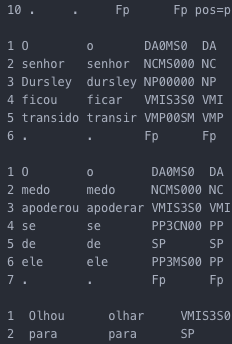
\includegraphics[scale=0.6]{analise1.png}
\caption{Exemplo de dois extratos no ficheiro harrypotter1.}
\label{img:analise1}
\end{figure}

\subsection{Personagens do Harry Potter}
\label{subsec:analise2}

///////////////////////// POR FAZER /////////////////////



\subsection{Palavras por Classes em HTML}

A terceira alínea do exercício requeria que fosse criado um filtro capaz de calcular uma lista de verbos, substantivos, adjectivos e advérbios. Consequentemente deveria ser colocado num ficheiro HTML cada uma destas listas.

Numa primeira abordagem ao problema foram analisadas as possíveis formas de apresentação de cada classe de palavras a serem filtradas.

Atendendo ao formato Freeling dum ficheiro CORPORA, foram de fácil verificação os seguintes factos, relativos à 6ª coluna de cada extrato:

\begin{enumerate}
 \item Se uma palavra for um verbo, então "pos=verb" está contido neste campo;
 \item Se uma palavra for um substantivo, então "pos=noun" está contido neste campo;
 \item Se uma palavra for um adjetivo, então "pos=adjective" está contido neste campo;
 \item Se uma palavra for um advérbio, então "pos=adverb" está contido neste campo;
\end{enumerate}

Foram ainda necessárias criar algumas bases na linguagem de programação HTML relativas à estruturação dum ficheiro, à criação dum cabeçalho e à listagens de elementos. Estas foram basicamente todas as operações necessárias, usadas nesta linguagem, para a realização desta alínea.


\subsection{Dicionário}

Nesta quarta alínea do exercício era requerida a apresentação de um dicionário implícito num ficheiro corpora. Este dicionário deve conter as lemas, as palavras derivadas das lemas, e a informação relativa a essas mesmas palavras. Esta informação vem dividida em colunas.

Realizando a análise de cada ficheiro concluímos que, para a resolução deste exercício o que nos interessava era:

\begin{itemize}
 \item Segunda coluna $\Rightarrow$ Palavra
 \item Terceira coluna $\Rightarrow$ Lema da Palavra
 \item Sexta coluna $\Rightarrow$ Informação da Palavra
\end{itemize}

\vspace{0.5cm}

Na figura \ref{img:analise4} é possivel verificar:

\begin{enumerate}
	\item Palavra $\Rightarrow$ Dumbledore ; Lema $\Rightarrow$ dumbledore ; Informação $\Rightarrow$ Noun Proper ;
	\item Palavra $\Rightarrow$ voltou ; Lema $\Rightarrow$ voltar ; Informação $\Rightarrow$ Verb Main Indicative Past 3 Singular ;
	\item Palavra $\Rightarrow$ se ; Lema $\Rightarrow$ se ; Informação $\Rightarrow$ Pronoun Personal 3 Common Invariable ;
	\item Palavra $\Rightarrow$ e ; Lema $\Rightarrow$ e ; Informação $\Rightarrow$ Conjunction Coordinating ;
	\item Palavra $\Rightarrow$ desceu ; Lema $\Rightarrow$ descer ; Informação $\Rightarrow$ Verb Main Indicative Past 3 Singular ;
	\item Palavra $\Rightarrow$ a ; Lema $\Rightarrow$ o ; Informação $\Rightarrow$ Determiner Article Feminine Singular ;
	\item Palavra $\Rightarrow$ rua ; Lema $\Rightarrow$ rua ; Informação $\Rightarrow$ Noun Common Feminine Singular ;
	\item Palavra $\Rightarrow$ . ; Lema $\Rightarrow$ . ; Informação $\Rightarrow$ Punctuation Period ;
\end{enumerate}


\begin{figure}[H]
\centering
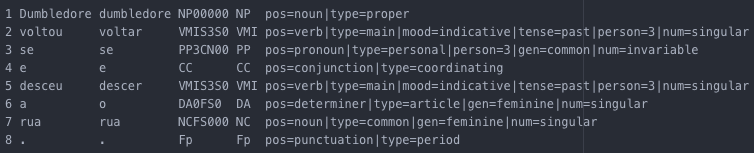
\includegraphics[scale=0.6]{analise4.png}
\caption{Exemplo de um extrato no ficheiro harrypotter1.}
\label{img:analise4}
\end{figure}


\chapter{Conceção/desenho da Resolução}
\label{chap:concecao}

///////////////////////// A REVER E A ACRESCENTAR ALGO /////////////////////

Neste capítulo baseando-nos nas análises feitas aos ficheiros que serviram de input ao filtros, construímos os algoritmos para a resolução de cada alínea requisitada no enunciado.

\section{Algoritmos}
\subsection{Número de Extratos}

///////////////////////// POR FAZER /////////////////////


\subsection{Personagens do Harry Potter}
\label{sub:algoritmos2}

///////////////////////// POR FAZER /////////////////////


\subsection{Palavras por Classes em HTML}
\label{sub:algoritmos3}

Inicialmente no bloco de \textbf{BEGIN} não alteramos nada que fosse relativo ao \textbf{Register Separator}, nem ao \textbf{Field Separator}, pelo que os valores associados a estes campos se mantiveram os pré-definidos. Neste bloco é realizada a criação duma pasta \textbf{C\_HTML} que albergará todos os ficheiros HTML necessários, e ainda é criado o ficheiro \textit{index.html} que corresponde ao ficheiro que é um índice de redirecionamento para outros.

Consoante a análise realizada no capítulo anterior, a parte do uso de expressões regulares para a filtragem das classes de palavras ficou facilitada uma vez que foi preciso apenas descriminar cada caso existente, todos eles relacionado com o 6º campo de cada registo. As expressões utilizadas foram as seguintes:

\begin{itemize}
	\item \$6 $\sim$ /pos=verb/
	\item \$6 $\sim$ /pos=adjective/
	\item \$6 $\sim$ /pos=adverb/ 
	\item \$6 $\sim$ /pos=noun/
\end{itemize}

Consoante cada classe, cada palavra filtrada era inserida num array associativo correspondente.

Finalmente no bloco de \textbf{END} é tratada a maior parte da construção de ficheiros HTML, e inserido nestes tudo o que foi filtrado. Criámos então 3 funções em AWK para se responsabilizarem desta tarefa. Estas são:

\begin{itemize}
	\item make\_page\_html(arg)
	\begin{itemize}
		\item Esta função é responsável pela criação dum ficheiro, cujo nome é passado como parâmetro (arg), e do seu cabeçalho.
	\end{itemize}
	\item list\_elem\_html(elem,filename)
	\begin{itemize}
		\item Esta função é responsável por adicionar ao ficheiro, cujo nome é passado como parâmetro (filename), um elemento a ser listado, também passado em argumento (elem).
	\end{itemize}
	\item make\_end\_html(arg)
	\begin{itemize}
		\item Esta função é responsável por terminar o ficheiro, cujo nome é passado como parâmetro (arg).
	\end{itemize}
\end{itemize}

As funções \textbf{make\_page\_html(arg)} e \textbf{make\_end\_html(arg)} são usadas somente uma vez. Entre elas é realizado um ciclo que percorre o array associativo correspondente, e ao ficheiro respetivo é adicionado o elemento que reside no array através da função \textbf{list\_elem\_html(elem,filename)}


\subsection{Dicionário}
\label{sub:algoritmos4}

///////////////////////// POR FAZER /////////////////////


\chapter{Codificação e Testes}
\label{chap:codificacao}

Para a presente secção de codificação e testes baseámo-nos nos capítulos anteriores, pois ambos são extremamente importantes para uma boa implementação desta fase. O capítulo de análise teve a sua relevância pois permitiu-nos ter já uma ideia de que expressões regulares utilizar para filtrar o que desejávamos e o capítulo da conceção da resolução foi relevante pois definimos os algoritmos necessários para coordenar o processo de filtragem para cada requisito.

\section{Estruturas de Dados}

\subsection{Número de Extratos}
///////////////////////// POR FAZER /////////////////////

\subsection{Personagens do Harry Potter}
///////////////////////// POR FAZER /////////////////////

\subsection{Palavras por classes em HTML}

Na terceira alínea foi necessário utilizar fundamentalmente uma estrutura de dados que já vem implementada em \textbf{AWK}, que são os \textbf{arrays associativos}. Foram de imensa utilidade uma vez que mapeiam todos os elementos necessários sem os repetirem.

Para esta alínea utilizamos 4 arrays deste género cada um para cada classe de palavras (verbos, substantivos, adjetivos e advérbios).

\subsection{Dicionário}
///////////////////////// POR FAZER /////////////////////

\section{Alternativas, Decisões e Problemas de Implementação}

\subsection{Número de Extratos}

///////////////////////// POR FAZER /////////////////////

Ao implementar esta questão começou-se por reparar que nem todas as páginas de autor estão de facto identificadas por um autor. Desta forma foi necessário ignorar todas as páginas de autor que não fossem identificadas por um autor que tivesse um nome com tamanho superior a 1.

O maior problema neste filtro foi identificar todas as formas como uma citação acabava e gerir esta questão. Encontrámos ao todo 10 formas diferentes de término duma citação e alguns dos casos são muito parecidos, de facto são especializações de casos mais gerais, pelo que a tarefa de encontrar o término duma citação ficou dificultada.

A propriedade \emph{longest match} do \textbf{flex}, foi outro entrave à implementação uma vez que como tínhamos casos que eram especialização de outros, muitas vezes o caso que era o \emph{longest match} não era o que era pretendido que fosse apanhado. Esta é a razão pela qual aparecem \textbf{\&quot;} no final de algumas citações.

Muita vezes fomo-nos deparando com citações que continham \textbf{\&quot;} não no final mas sim no meio das citações. Decidimos considerar que estes "tokens"  fariam parte da citação uma vez que apanhámos a citação toda até uma situação de término, ignorando o conteúdo de cada citação.

Para a realização deste filtro utilizámos as estruturas descritas acima em conjunto com algumas funções auxiliares que no permitiam inserir citações, autores, e ainda imprimir todas as citações da estrutura existente.


\subsection{Personagens do Harry Potter}

///////////////////////// POR FAZER /////////////////////

Tendo em conta a grande variedade de marcas para representar provérbios em diferentes países, a resolução desta questão foi condicionada por tal. Desta forma, são muitos os estados criados para as mesmas partes de diferentes páginas do ficheiro.

Após a análise explicada na secção \ref{subsec:analise2} foi possível concluir quais seriam os casos mais críticos. São exemplo disso os provérbios russos, que têm como marca inicial apenas \underline{*}. Devido à elevada ocorrência desta marca em todo o ficheiro, foi necessário limitar a filtragem com esta marca apenas à parte do ficheiro que pretendiamos, e tal foi possível através do conceito de Estado.

Relembrando o autómato apresentado na secção \ref{sub:algoritmos2}, existem quatro fases importantes no algoritmo.

Na fase inicial vamos percorrer as páginas do ficheiro. Na segunda fase vamos interpretar o título da página e, tendo em conta o resultado obtido, o estado seguinte vai ser diferente. Existe o caso \textit{default} que apanha tudo o que aparece em frente à palavra \textit{Provérbios} mas, devido à grande variedade de marcas, tivemos aqui que forçar alguns processos a seguir caminhos particulares, sendo nesses casos a condição o título inteiro, como por exemplo \textit{Provérbios russos}.

A partir deste momento o estado passa a seguir um caminho particular, que é o \textit{CONTEUDO\_RUS}. Esta é, portanto, a terceira fase. Depois de estar no conteúdo russo e serem atingidas as marcas de início de provérbio, o estado passa a ser o \textit{QUOTE\_RUS}, que vai ler a citação e, de seguida, imprimi-la no ecrã com a formatação desejada. Esta quarta fase regressa depois ao conteúdo da página de provérbios russos para continuar a sua filtragem.

Após a análise total das páginas, e de forma a não ter contextos em exagero, tentamos unificar num só contexto os países que teriam as mesmas marcas, ou marcas que fossem compatíveis. São exemplos deste facto os provérbios turcos, búlgaros, chineses e holandeses, que são compatíveis e deram origem aos estados CONTEUDO\_TURQ\_BUL\_CHI\_HOL e QUOTE\_TURQ\_BUL\_CHI\_HOL.


\newpage

\subsection{Dicionário}

///////////////////////// POR FAZER /////////////////////


\section{Testes realizados e Resultados}
\subsection{Número de Extratos}

Aplicando o filtro criado para a primeira questão com qualquer um dos ficheiros de input disponibilizados, verificam-se resultados com um formato como o da seguinte imagem.

A informação fornecido é o número de extratos.

\begin{figure}[H]
\centering

\includegraphics[scale=0.7]{testes1.png}
\caption{Resultado do filtro 1 para o ficheiro fl0.}
\label{img:testes1}
\end{figure}


\subsection{Lista de Provérbios}

///////////////////////// POR FAZER /////////////////////

Tendo em conta a imensa variedade de marcas de início de provérbios, nesta fase os testes tiveram uma enorme importância.

O resultado do filtro está organizado por Título e Citações, sendo que no final é apresentada uma estatística da filtragem, que contempla o número de páginas total, o número de páginas com título começado por 'Provérbios', e o número de citações recolhidas no filtro.

Seguem-se alguns exemplos de provérbios obtidos da filtragem.


\newpage

\subsection{Palavras por Classes em HTML}

O resultado do filtro criado e executado com algum dos ficheiros de input é a criação duma pasta \textbf{C\_HTML} que contém 5 ficheiros HTML. Um destes ficheiros funciona como um índice (\textbf{index.html}) que redireciona para outras páginas HTML. Todos os restantes ficheiros contêm uma lista, ou de verbos, ou de substantivos, ou de adjetivos, ou ainda de advérbios.

A seguir são apresentadas algumas imagens dos resultados em páginas num browser.

\begin{figure}[H]
\centering
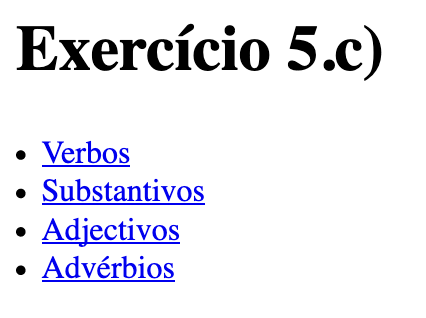
\includegraphics[scale=0.6]{index.png}
\caption{índice criado.}
\label{img:index}
\end{figure}

Carregando em algum dos elementos listados, redireciona-nos para outra página HTML do género das seguintes.

\begin{figure}[H]
\centering
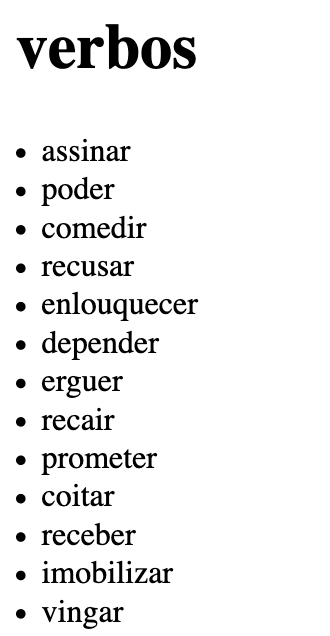
\includegraphics[scale=0.6]{verbos.png}
\caption{Exemplo dum ficheiro com uma lista de verbos.}
\label{img:verbos}
\end{figure}

\begin{figure}[H]
\centering
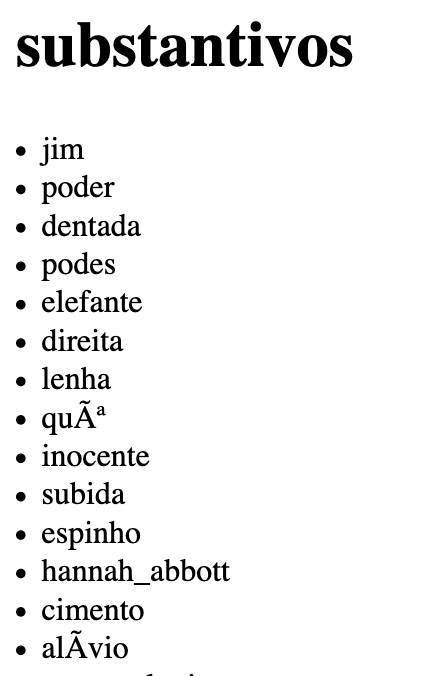
\includegraphics[scale=0.6]{substantivos.png}
\caption{Exemplo dum ficheiro com uma lista de substantivos.}
\label{img:substantivos}
\end{figure}

\begin{figure}[H]
\centering
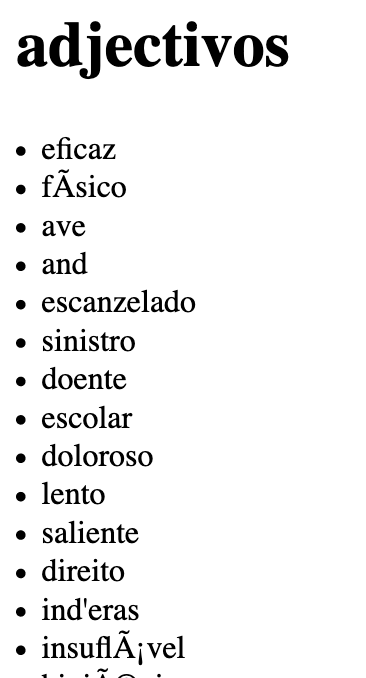
\includegraphics[scale=0.6]{adjetivos.png}
\caption{Exemplo dum ficheiro com uma lista de adjetivos.}
\label{img:adjetivos}
\end{figure}

\begin{figure}[H]
\centering
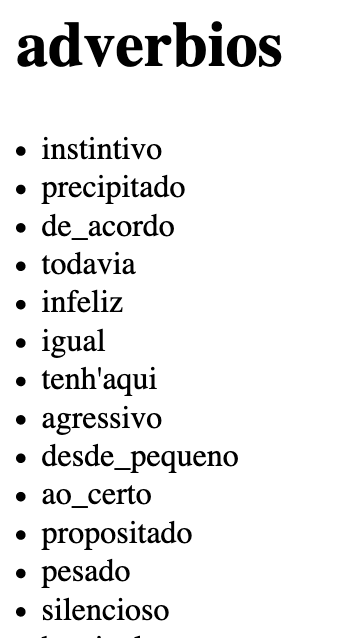
\includegraphics[scale=0.6]{adverbios.png}
\caption{Exemplo dum ficheiro com uma lista de adverbios.}
\label{img:adverbios}
\end{figure}

\newpage

\subsection{Dicionário}

A seguinte imagem apresenta um excerto do resultado do filtro que constrói um dicionário com base num dos ficheiros escolhidos como parâmetro.

O dicionário, conforme pode ser verificado, é apresentado por ordem alfabética, e cada uma das palavras derivadas contêm a sua informação morfossintática.

\begin{figure}[H]
\centering
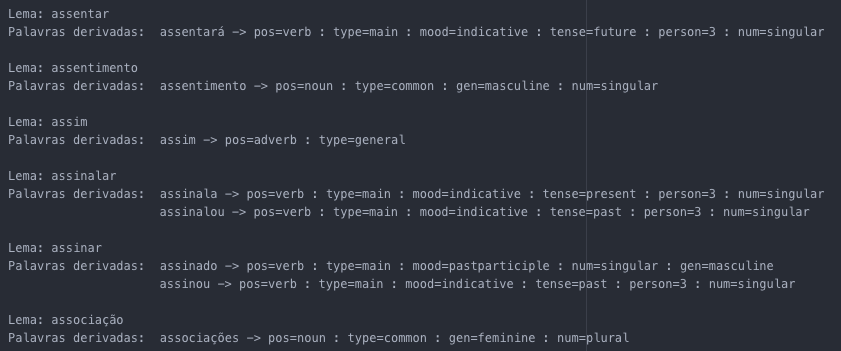
\includegraphics[scale=0.5]{testes4.png}
\caption{Excerto do resultado do filtro 4 para o ficheiro fl1.}
\label{img:testes4}
\end{figure}


\chapter{Extras}
\label{chap:extras}




\chapter{Conclusão}
\label{chap:concl}

///////////////////////// POR FAZER /////////////////////

Tendo em conta os requisitos deste projeto, e o trabalho realizado pelo grupo, achamos que os objetivos fundamentais foram atingidos, sendo estes a capacidade de criar padrões com uso de \textbf{Expressões Regulares}, o entendimento da utilização da ferramenta \textbf{flex} para a criação destes padrões, a capacidade de analisar ficheiros de entrada e criar algoritmos de resolução recorrendo a \textbf{autómatos}.

Ao longo da realização deste projeto o grupo encontrou várias dificuldades, estando estas relacionadas maioritariamente com a quantidade de formas diferentes em que apareciam as citações e os provérbios a serem filtrados. Entendemos portanto, que esta foi a maior dificuldade pois foi necessário a agilização dos membros do grupo para encontrarem soluções para a filtragem de certos padrões.

Em jeito de conclusão o grupo acha que todas as alíneas requisitadas no enunciado foram terminadas com sucesso, e os objetivos principais deste projeto foram atingidos.


\end{document}
